% Options for packages loaded elsewhere
% Options for packages loaded elsewhere
\PassOptionsToPackage{unicode}{hyperref}
\PassOptionsToPackage{hyphens}{url}
\PassOptionsToPackage{dvipsnames,svgnames,x11names}{xcolor}
%
\documentclass[
  letterpaper,
  DIV=11,
  numbers=noendperiod]{scrartcl}
\usepackage{xcolor}
\usepackage{amsmath,amssymb}
\setcounter{secnumdepth}{-\maxdimen} % remove section numbering
\usepackage{iftex}
\ifPDFTeX
  \usepackage[T1]{fontenc}
  \usepackage[utf8]{inputenc}
  \usepackage{textcomp} % provide euro and other symbols
\else % if luatex or xetex
  \usepackage{unicode-math} % this also loads fontspec
  \defaultfontfeatures{Scale=MatchLowercase}
  \defaultfontfeatures[\rmfamily]{Ligatures=TeX,Scale=1}
\fi
\usepackage{lmodern}
\ifPDFTeX\else
  % xetex/luatex font selection
\fi
% Use upquote if available, for straight quotes in verbatim environments
\IfFileExists{upquote.sty}{\usepackage{upquote}}{}
\IfFileExists{microtype.sty}{% use microtype if available
  \usepackage[]{microtype}
  \UseMicrotypeSet[protrusion]{basicmath} % disable protrusion for tt fonts
}{}
\makeatletter
\@ifundefined{KOMAClassName}{% if non-KOMA class
  \IfFileExists{parskip.sty}{%
    \usepackage{parskip}
  }{% else
    \setlength{\parindent}{0pt}
    \setlength{\parskip}{6pt plus 2pt minus 1pt}}
}{% if KOMA class
  \KOMAoptions{parskip=half}}
\makeatother
% Make \paragraph and \subparagraph free-standing
\makeatletter
\ifx\paragraph\undefined\else
  \let\oldparagraph\paragraph
  \renewcommand{\paragraph}{
    \@ifstar
      \xxxParagraphStar
      \xxxParagraphNoStar
  }
  \newcommand{\xxxParagraphStar}[1]{\oldparagraph*{#1}\mbox{}}
  \newcommand{\xxxParagraphNoStar}[1]{\oldparagraph{#1}\mbox{}}
\fi
\ifx\subparagraph\undefined\else
  \let\oldsubparagraph\subparagraph
  \renewcommand{\subparagraph}{
    \@ifstar
      \xxxSubParagraphStar
      \xxxSubParagraphNoStar
  }
  \newcommand{\xxxSubParagraphStar}[1]{\oldsubparagraph*{#1}\mbox{}}
  \newcommand{\xxxSubParagraphNoStar}[1]{\oldsubparagraph{#1}\mbox{}}
\fi
\makeatother

\usepackage{color}
\usepackage{fancyvrb}
\newcommand{\VerbBar}{|}
\newcommand{\VERB}{\Verb[commandchars=\\\{\}]}
\DefineVerbatimEnvironment{Highlighting}{Verbatim}{commandchars=\\\{\}}
% Add ',fontsize=\small' for more characters per line
\usepackage{framed}
\definecolor{shadecolor}{RGB}{241,243,245}
\newenvironment{Shaded}{\begin{snugshade}}{\end{snugshade}}
\newcommand{\AlertTok}[1]{\textcolor[rgb]{0.68,0.00,0.00}{#1}}
\newcommand{\AnnotationTok}[1]{\textcolor[rgb]{0.37,0.37,0.37}{#1}}
\newcommand{\AttributeTok}[1]{\textcolor[rgb]{0.40,0.45,0.13}{#1}}
\newcommand{\BaseNTok}[1]{\textcolor[rgb]{0.68,0.00,0.00}{#1}}
\newcommand{\BuiltInTok}[1]{\textcolor[rgb]{0.00,0.23,0.31}{#1}}
\newcommand{\CharTok}[1]{\textcolor[rgb]{0.13,0.47,0.30}{#1}}
\newcommand{\CommentTok}[1]{\textcolor[rgb]{0.37,0.37,0.37}{#1}}
\newcommand{\CommentVarTok}[1]{\textcolor[rgb]{0.37,0.37,0.37}{\textit{#1}}}
\newcommand{\ConstantTok}[1]{\textcolor[rgb]{0.56,0.35,0.01}{#1}}
\newcommand{\ControlFlowTok}[1]{\textcolor[rgb]{0.00,0.23,0.31}{\textbf{#1}}}
\newcommand{\DataTypeTok}[1]{\textcolor[rgb]{0.68,0.00,0.00}{#1}}
\newcommand{\DecValTok}[1]{\textcolor[rgb]{0.68,0.00,0.00}{#1}}
\newcommand{\DocumentationTok}[1]{\textcolor[rgb]{0.37,0.37,0.37}{\textit{#1}}}
\newcommand{\ErrorTok}[1]{\textcolor[rgb]{0.68,0.00,0.00}{#1}}
\newcommand{\ExtensionTok}[1]{\textcolor[rgb]{0.00,0.23,0.31}{#1}}
\newcommand{\FloatTok}[1]{\textcolor[rgb]{0.68,0.00,0.00}{#1}}
\newcommand{\FunctionTok}[1]{\textcolor[rgb]{0.28,0.35,0.67}{#1}}
\newcommand{\ImportTok}[1]{\textcolor[rgb]{0.00,0.46,0.62}{#1}}
\newcommand{\InformationTok}[1]{\textcolor[rgb]{0.37,0.37,0.37}{#1}}
\newcommand{\KeywordTok}[1]{\textcolor[rgb]{0.00,0.23,0.31}{\textbf{#1}}}
\newcommand{\NormalTok}[1]{\textcolor[rgb]{0.00,0.23,0.31}{#1}}
\newcommand{\OperatorTok}[1]{\textcolor[rgb]{0.37,0.37,0.37}{#1}}
\newcommand{\OtherTok}[1]{\textcolor[rgb]{0.00,0.23,0.31}{#1}}
\newcommand{\PreprocessorTok}[1]{\textcolor[rgb]{0.68,0.00,0.00}{#1}}
\newcommand{\RegionMarkerTok}[1]{\textcolor[rgb]{0.00,0.23,0.31}{#1}}
\newcommand{\SpecialCharTok}[1]{\textcolor[rgb]{0.37,0.37,0.37}{#1}}
\newcommand{\SpecialStringTok}[1]{\textcolor[rgb]{0.13,0.47,0.30}{#1}}
\newcommand{\StringTok}[1]{\textcolor[rgb]{0.13,0.47,0.30}{#1}}
\newcommand{\VariableTok}[1]{\textcolor[rgb]{0.07,0.07,0.07}{#1}}
\newcommand{\VerbatimStringTok}[1]{\textcolor[rgb]{0.13,0.47,0.30}{#1}}
\newcommand{\WarningTok}[1]{\textcolor[rgb]{0.37,0.37,0.37}{\textit{#1}}}

\usepackage{longtable,booktabs,array}
\newcounter{none} % for unnumbered tables
\usepackage{calc} % for calculating minipage widths
% Correct order of tables after \paragraph or \subparagraph
\usepackage{etoolbox}
\makeatletter
\patchcmd\longtable{\par}{\if@noskipsec\mbox{}\fi\par}{}{}
\makeatother
% Allow footnotes in longtable head/foot
\IfFileExists{footnotehyper.sty}{\usepackage{footnotehyper}}{\usepackage{footnote}}
\makesavenoteenv{longtable}
\usepackage{graphicx}
\makeatletter
\newsavebox\pandoc@box
\newcommand*\pandocbounded[1]{% scales image to fit in text height/width
  \sbox\pandoc@box{#1}%
  \Gscale@div\@tempa{\textheight}{\dimexpr\ht\pandoc@box+\dp\pandoc@box\relax}%
  \Gscale@div\@tempb{\linewidth}{\wd\pandoc@box}%
  \ifdim\@tempb\p@<\@tempa\p@\let\@tempa\@tempb\fi% select the smaller of both
  \ifdim\@tempa\p@<\p@\scalebox{\@tempa}{\usebox\pandoc@box}%
  \else\usebox{\pandoc@box}%
  \fi%
}
% Set default figure placement to htbp
\def\fps@figure{htbp}
\makeatother





\setlength{\emergencystretch}{3em} % prevent overfull lines

\providecommand{\tightlist}{%
  \setlength{\itemsep}{0pt}\setlength{\parskip}{0pt}}



 


\KOMAoption{captions}{tableheading}
\makeatletter
\@ifpackageloaded{caption}{}{\usepackage{caption}}
\AtBeginDocument{%
\ifdefined\contentsname
  \renewcommand*\contentsname{Table of contents}
\else
  \newcommand\contentsname{Table of contents}
\fi
\ifdefined\listfigurename
  \renewcommand*\listfigurename{List of Figures}
\else
  \newcommand\listfigurename{List of Figures}
\fi
\ifdefined\listtablename
  \renewcommand*\listtablename{List of Tables}
\else
  \newcommand\listtablename{List of Tables}
\fi
\ifdefined\figurename
  \renewcommand*\figurename{Figure}
\else
  \newcommand\figurename{Figure}
\fi
\ifdefined\tablename
  \renewcommand*\tablename{Table}
\else
  \newcommand\tablename{Table}
\fi
}
\@ifpackageloaded{float}{}{\usepackage{float}}
\floatstyle{ruled}
\@ifundefined{c@chapter}{\newfloat{codelisting}{h}{lop}}{\newfloat{codelisting}{h}{lop}[chapter]}
\floatname{codelisting}{Listing}
\newcommand*\listoflistings{\listof{codelisting}{List of Listings}}
\makeatother
\makeatletter
\makeatother
\makeatletter
\@ifpackageloaded{caption}{}{\usepackage{caption}}
\@ifpackageloaded{subcaption}{}{\usepackage{subcaption}}
\makeatother
\usepackage{bookmark}
\IfFileExists{xurl.sty}{\usepackage{xurl}}{} % add URL line breaks if available
\urlstyle{same}
% fallback for those not using the hyperref driver hyperxmp:
\makeatletter
\@ifundefined{xmpquote}{\newcommand{\xmpquote}[1]{#1}}{}
\makeatother
\hypersetup{
  pdftitle={Homework Assignment 1},
  pdfauthor={Karla V. Ramos},
  colorlinks=true,
  linkcolor={blue},
  filecolor={Maroon},
  citecolor={Blue},
  urlcolor={Blue},
  pdfcreator={LaTeX via pandoc}}


\title{Homework Assignment 1}
\usepackage{etoolbox}
\makeatletter
\providecommand{\subtitle}[1]{% add subtitle to \maketitle
  \apptocmd{\@title}{\par {\large #1 \par}}{}{}
}
\makeatother
\subtitle{Mapping the Relationship Between Socioeconomic Vulnerability
and Wastewater Discharge in the San Joaquin County}
\author{Karla V. Ramos}
\date{2026-10-09}
\begin{document}
\maketitle


\begin{Shaded}
\begin{Highlighting}[]
\FunctionTok{library}\NormalTok{(tidyverse)}
\FunctionTok{library}\NormalTok{(sf)}
\FunctionTok{library}\NormalTok{(here)}
\FunctionTok{library}\NormalTok{(tmap)}

\CommentTok{\# Read in geodatabase of EJScreen data at the Census Block Group level}
\NormalTok{ejscreen }\OtherTok{\textless{}{-}}\NormalTok{ sf}\SpecialCharTok{::}\FunctionTok{st\_read}\NormalTok{(here}\SpecialCharTok{::}\FunctionTok{here}\NormalTok{(}\StringTok{"data"}\NormalTok{, }\StringTok{"ejscreen"}\NormalTok{,}\StringTok{"EJSCREEN\_2023\_BG\_StatePct\_with\_AS\_CNMI\_GU\_VI.gdb"}\NormalTok{)) }
\end{Highlighting}
\end{Shaded}

\begin{verbatim}
Reading layer `EJSCREEN_StatePctiles_with_AS_CNMI_GU_VI' from data source 
  `/Users/karlaramos/Desktop/Git/eds223-HW/EDS223-HW1/data/ejscreen/EJSCREEN_2023_BG_StatePct_with_AS_CNMI_GU_VI.gdb' 
  using driver `OpenFileGDB'
Simple feature collection with 243021 features and 223 fields
Geometry type: MULTIPOLYGON
Dimension:     XY
Bounding box:  xmin: -19951910 ymin: -1617130 xmax: 16259830 ymax: 11554350
Projected CRS: WGS 84 / Pseudo-Mercator
\end{verbatim}

\begin{Shaded}
\begin{Highlighting}[]
\CommentTok{\# Filter to California}
\NormalTok{california }\OtherTok{\textless{}{-}}\NormalTok{ ejscreen }\SpecialCharTok{\%\textgreater{}\%}
\NormalTok{  dplyr}\SpecialCharTok{::}\FunctionTok{filter}\NormalTok{(ST\_ABBREV }\SpecialCharTok{==} \StringTok{"CA"}\NormalTok{) }

\CommentTok{\# filter to San Joaquin County}
\NormalTok{san\_joaquin }\OtherTok{\textless{}{-}}\NormalTok{ ejscreen }\SpecialCharTok{\%\textgreater{}\%}
\NormalTok{  dplyr}\SpecialCharTok{::}\FunctionTok{filter}\NormalTok{(CNTY\_NAME }\SpecialCharTok{\%in\%} \FunctionTok{c}\NormalTok{(}\StringTok{"San Joaquin County"}\NormalTok{))}

\CommentTok{\# Find the average values for all variables within counties}
\NormalTok{california\_counties }\OtherTok{\textless{}{-}} \FunctionTok{aggregate}\NormalTok{(california, }\AttributeTok{by =} \FunctionTok{list}\NormalTok{(california}\SpecialCharTok{$}\NormalTok{CNTY\_NAME), }\AttributeTok{FUN =}\NormalTok{ mean)}
\end{Highlighting}
\end{Shaded}

\begin{Shaded}
\begin{Highlighting}[]
\NormalTok{sj\_waterdischarge }\OtherTok{\textless{}{-}}\FunctionTok{tm\_shape}\NormalTok{(san\_joaquin)}\SpecialCharTok{+}  
  \FunctionTok{tm\_title}\NormalTok{(}\StringTok{\textquotesingle{}Waterwater Discharge in San Joaquin County (2023)\textquotesingle{}}\NormalTok{)}\SpecialCharTok{+}
  \FunctionTok{tm\_polygons}\NormalTok{(}\AttributeTok{fill=} \StringTok{\textquotesingle{}P\_PWDIS\textquotesingle{}}\NormalTok{, }\AttributeTok{fill.legend =} \FunctionTok{tm\_legend}\NormalTok{(}\AttributeTok{title =} \StringTok{"Toxicity{-}weighted concentration / km"}\NormalTok{))}\SpecialCharTok{+} \CommentTok{\#within polygons you add title for legend}
  \FunctionTok{tm\_add\_legend}\NormalTok{(}\AttributeTok{type =} \StringTok{"line"}\NormalTok{, }\AttributeTok{col =} \StringTok{"white"}\NormalTok{) }\SpecialCharTok{+}
  \FunctionTok{tm\_layout}\NormalTok{(}\AttributeTok{bg.color =} \StringTok{"white"}\NormalTok{)}\SpecialCharTok{+}
  \FunctionTok{tm\_style}\NormalTok{(}\StringTok{"white"}\NormalTok{) }\SpecialCharTok{+}
  \FunctionTok{tm\_compass}\NormalTok{() }\SpecialCharTok{+}
  \FunctionTok{tm\_scalebar}\NormalTok{() }\CommentTok{\#percentile of wastewater discharge}
\end{Highlighting}
\end{Shaded}

\begin{Shaded}
\begin{Highlighting}[]
\CommentTok{\# A Demographic Index is based on the average of two demographic indicators; Percent Low{-}Income and Percent Minority.}
\NormalTok{sj\_demographic }\OtherTok{\textless{}{-}} \FunctionTok{tm\_shape}\NormalTok{(san\_joaquin)}\SpecialCharTok{+} \CommentTok{\# defines the spacial object to plot }
    \FunctionTok{tm\_polygons}\NormalTok{(}\AttributeTok{fill=} \StringTok{\textquotesingle{}P\_DEMOGIDX\_5\textquotesingle{}}\NormalTok{, }\AttributeTok{fill.legend =} \FunctionTok{tm\_legend}\NormalTok{(}\AttributeTok{title =} \StringTok{"Average of percent}
\StringTok{low income and percent people of color"}\NormalTok{)) }\SpecialCharTok{+}
    \FunctionTok{tm\_title}\NormalTok{(}\StringTok{\textquotesingle{}EJ Demographic Index in San Joaquin County (2023)\textquotesingle{}}\NormalTok{)}\SpecialCharTok{+}
    \FunctionTok{tm\_add\_legend}\NormalTok{(}\AttributeTok{type =} \StringTok{"line"}\NormalTok{, }\AttributeTok{col =} \StringTok{"white"}\NormalTok{) }\SpecialCharTok{+}
    \FunctionTok{tm\_layout}\NormalTok{(}\AttributeTok{bg.color =} \StringTok{"white"}\NormalTok{)}\SpecialCharTok{+}
    \FunctionTok{tm\_style}\NormalTok{(}\StringTok{"beaver"}\NormalTok{) }\SpecialCharTok{+}
    \FunctionTok{tm\_compass}\NormalTok{(}\AttributeTok{type =}\StringTok{"arrow"}\NormalTok{) }\SpecialCharTok{+}
    \FunctionTok{tm\_scalebar}\NormalTok{() }\CommentTok{\#percentile of wastewater discharge}
\end{Highlighting}
\end{Shaded}

\begin{Shaded}
\begin{Highlighting}[]
\FunctionTok{tmap\_arrange}\NormalTok{(sj\_waterdischarge, sj\_demographic)}
\end{Highlighting}
\end{Shaded}

\pandocbounded{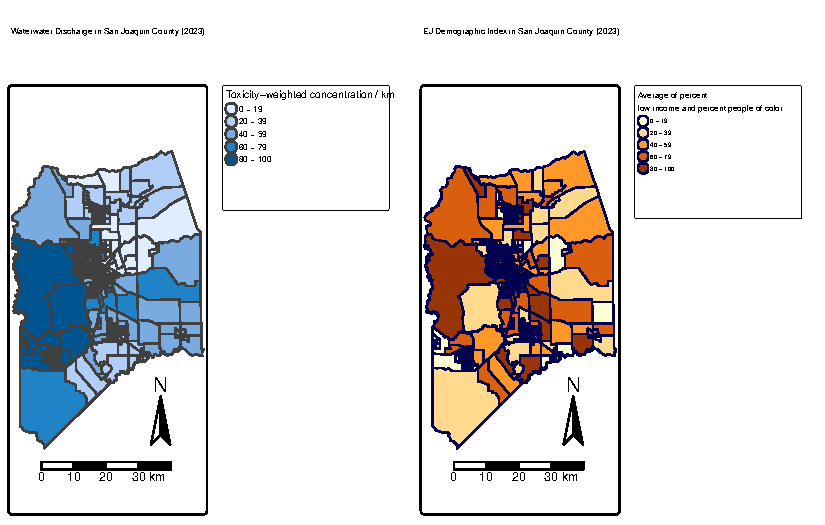
\includegraphics[keepaspectratio]{ej_screen_files/figure-pdf/unnamed-chunk-4-1.pdf}}

\subsection{Mapping purpose:}\label{mapping-purpose}

In San Joaquin County, unsafe water quality poses a major public health
threat, particularly for communities identified by EJScreen's
demographic indicators. Water contamination and toxicity have been
linked to agricultural and industrial activity, but the full scope of
exposure is difficult to measure because much of the available data does
not account for people who travel through, recreate in, or work near
contaminated water.

The map on the left (Wastewater Discharge in San Joaquin County, 2023)
shows wastewater discharge from permitted facilities, measured as
toxicity-weighted concentration divided by distance in meters. The map
on the right (EJ Demographic Index in San Joaquin County, 2023) shows a
demographic index based on percent low-income and percent people of
color. In the western part of the county, areas with high wastewater
toxicity substantially overlap with areas scoring high on the
demographic index.




\end{document}
